% =====================================================================
%  Introduction to Deep Learning — Class 13
%  Topic (course plan): Deep Networks
%  Subtopic (course plan): Gradient Descent and optimization
%  Sources (course plan): Bishop Chapter 7, Prince Chapters 6-7
%
%  Narrative order: the convex case first, in full, then exactly what
%  breaks when the loss stops being convex, then the fix.  See
%  _shared/PLAN_Classes13_14_15.md for how Bishop Ch.7 and Prince
%  Ch.6-7 are divided between Classes 13, 14 and 15.
%
%  Figures: the published figures from each textbook's own repository.
%  Points the books illustrate with no figure are stated without one;
%  the B variant supplies purpose-built figures for those.
%
%  Compile:  xelatex main.tex   (run twice)
% =====================================================================
\documentclass[aspectratio=169, 11pt]{beamer}

\usetheme{metropoliscustom}

\usepackage{graphicx}
\DeclareGraphicsExtensions{.pdf,.png,.jpg}
\graphicspath{{figs_official/}{Class13_Gradient_Descent_Optimization/A_Textbook_Figures/figs_official/}}
\usepackage{amsmath, amssymb}
\usepackage{bm}
\usepackage{tikz}
\usetikzlibrary{arrows.meta, positioning, calc, decorations.pathreplacing,
                shapes.geometric}
\tcbuselibrary{skins}

\definecolor{shc}{HTML}{341651}
\definecolor{tealc}{HTML}{1C7293}
\definecolor{dpc}{HTML}{800000}
\definecolor{accc}{HTML}{B8860B}

% ---- theorem environments -------------------------------------------
\setbeamertemplate{theorems}[numbered]
\usepackage{remreset}
\makeatletter\@removefromreset{theorem}{section}\makeatother
\renewcommand{\thetheorem}{\arabic{theorem}}
\newtheorem{lemmax}[theorem]{Lemma}
\newtheorem{propx}[theorem]{Proposition}
\newtheorem{corx}[theorem]{Corollary}
\newtheorem{algox}[theorem]{Algorithm}

% ---- parallel strip: batch (left) vs stochastic (right) --------------
\newcommand{\bspar}[2]{%
  \vfill
  {\scriptsize
  \begin{tcolorbox}[enhanced, sidebyside, sidebyside align=top,
                    lefthand ratio=0.485,
                    segmentation style={shc!35, line width=0.6pt},
                    colback=shc!5, colframe=shc!35, boxrule=0.5pt,
                    arc=1.2mm, left=1.6mm, right=1.6mm,
                    top=0.6mm, bottom=0.6mm,
                    before skip=0pt, after skip=0pt]
    {\color{shc}\textbf{BATCH}}\hspace{0.55em}#1
  \tcblower
    {\color{dpc}\textbf{STOCHASTIC}}\hspace{0.55em}#2
  \end{tcolorbox}}%
  \vspace{0.35em}%
}

\newcommand{\bridge}[1]{%
  {\scriptsize\itshape\color{mcMuted} #1\par}\vspace{0.35em}}

% one small source line per slide, right-aligned at the foot
\newcommand{\srcline}[1]{%
  \par\vspace{0.25em}%
  {\scriptsize\color{mcMuted}\hfill #1\par}}

\newcommand{\figsource}[1]{{\scriptsize\color{mcMuted} #1}}
\newcommand{\figcap}[2][0.90]{%
  \begin{center}\begin{minipage}{#1\textwidth}\centering
    {\scriptsize\color{mcMuted} #2}
  \end{minipage}\end{center}}

% =====================================================================
\title{Deep Networks}
\subtitle{Gradient Descent and Optimization}
\author{Introduction to Deep Learning \ \textperiodcentered\ Class 13}
\institute{}
\date{}

\footleft{Introduction to Deep Learning}
\footright{Gradient Descent}
\titlelogos{}

\begin{document}

\maketitle

\begin{frame}{Outline}
  \tableofcontents
\end{frame}

% =====================================================================
\section{The Training Objective}
% =====================================================================

\begin{frame}{From the gradient to the step}
  \bridge{Class 11 ended with a gradient in hand. This class asks what to
  do with it.}
  \vspace{0.35em}
  {\footnotesize
  \renewcommand{\arraystretch}{1.35}
  \begin{tabular}{@{}l@{\hspace{1.4em}}l@{\hspace{1.4em}}l@{}}
    \textbf{Class} & \textbf{The question} & \textbf{The object}\\
    11 & How do we obtain $\nabla E$ at all? & the algorithm\\
    \textbf{13} & \textbf{What is the step, and does it go down?}
       & \textbf{the direction and its estimate}\\
    14 & How fast, and under what conditions? & the dynamics\\
    15 & How do we keep the signals well-scaled? & the conditioning\\
  \end{tabular}}
  \vspace{0.9em}

  \begin{redhighlight}
    Today's plan: start with a loss on which descent \emph{cannot} fail,
    understand exactly why, and then remove that assumption one piece at
    a time.
  \end{redhighlight}
\end{frame}

\begin{frame}{Notation}
  \vspace{0.35em}
  {\footnotesize
  \renewcommand{\arraystretch}{1.30}
  \begin{columns}[T, onlytextwidth]
    \begin{column}{0.49\textwidth}
      \begin{tabular}{@{}l@{\hspace{1.5em}}l@{}}
        $\mathbf{x}$, $y$, $\hat y$ & input, target, prediction\\
        $w$ & every learnable parameter\\
        $E(w)$ & the error function being minimized\\
        $E_n(w)$ & its contribution from point $n$\\
        $\nabla E$ & gradient of $E$ with respect to $w$\\
        $H$ & Hessian, $\nabla\nabla E$\\
      \end{tabular}
    \end{column}
    \begin{column}{0.49\textwidth}
      \begin{tabular}{@{}l@{\hspace{1.5em}}l@{}}
        $\eta$ & learning rate\\
        $\tau$ & iteration index\\
        $N$ & training-set size\\
        $B$ & mini-batch size\\
        $W$ & number of parameters\\
        $\lambda_i$, $u_i$ & eigenvalues, eigenvectors of $H$\\
      \end{tabular}
    \end{column}
  \end{columns}}
\end{frame}

\begin{frame}{The training objective}
  \vspace{-0.7em}
  \[
    \hat w = \arg\min_{w} E(w),
    \qquad
    E(w) = \sum_{n=1}^{N} E_n(w)
  \]
  \vspace{-1.0em}
  \begin{itemize}\itemsep0.35em
    \item Class 6 built $E(w)$ from maximum likelihood; Class 11 made
          $\nabla E$ computable
    \item $E$ is a \alert{sum over data points} because the likelihood of
          independent observations is a product
    \item No closed form solves $\nabla E(w) = 0$ for a network, so we
          iterate
  \end{itemize}
  \begin{redhighlight}
    Optimization is a means, not the goal: we want good predictions on
    \emph{new} data, so we will happily stop short of the exact minimum.
  \end{redhighlight}
  \srcline{Prince (2023), \S6.1; Bishop \& Bishop (2024), \S7.}
\end{frame}

\begin{frame}{The error surface}
  \begin{center}
    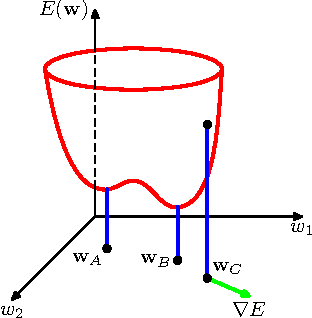
\includegraphics[height=0.55\textheight]{Bishop7_1}
  \end{center}
  \figcap[0.97]{$E$ viewed as a surface over weight space. $w_A$ is a
  local minimum and $w_B$ the global minimum; at $w_C$ the local slope
  is $\nabla E$. Bishop \& Bishop (2024), Fig.~7.1.}
\end{frame}

\begin{frame}{The hiker in fog}
  \vspace{0.35em}
  {\footnotesize
  \renewcommand{\arraystretch}{1.34}
  \begin{tabular}{@{}l@{\hspace{2.2em}}l@{}}
    \textbf{On the mountain} & \textbf{In training}\\
    the altitude at your feet & $E(w)$ at the current $w$\\
    the slope you can feel underfoot & $\nabla E(w)$\\
    fog: no view of the far side & no access to the global shape of $E$\\
    the length of one stride & the learning rate $\eta$\\
    the valley you happen to start in & the initialization\\
  \end{tabular}}
  \vspace{0.9em}

  \begin{itemize}\itemsep0.35em
    \item The hiker knows the slope \alert{exactly} and the map
          \alert{not at all}
    \item Every design choice today is about how far to trust one local
          slope reading
  \end{itemize}
\end{frame}

% =====================================================================
\section{Descent on a Convex Loss}
% =====================================================================

\begin{frame}{Convexity}
  \begin{block}{Definition (convex function)}
    $E$ is \alert{convex} if no chord lies below its graph:
    \[
      E\big(\theta u + (1-\theta) v\big)
        \;\leq\; \theta E(u) + (1-\theta) E(v)
      \qquad \forall\, u, v, \; \theta \in [0,1].
    \]
  \end{block}
  \vspace{0.4em}
  \begin{itemize}\itemsep0.4em
    \item Where $E$ is twice differentiable this says the Hessian $H$ is
          positive semi-definite \alert{everywhere}
    \item Least squares for a \alert{linear} model is convex
    \item So is logistic regression, and every generalised linear model
          of Class 6
  \end{itemize}
  \srcline{Prince (2023), \S6.1.2.}
\end{frame}

\begin{frame}{Convex and non-convex, side by side}
  \begin{center}
    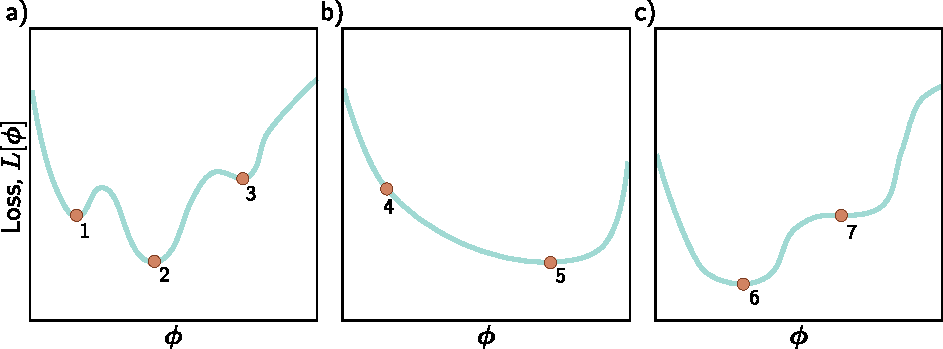
\includegraphics[height=0.55\textheight]{TrainConvexProb}
  \end{center}
  \figcap[0.97]{The chord test. On the left every chord lies above the graph; on the right a single chord cutting below is enough to disqualify the function. Prince (2023), \S6.1.2.}
\end{frame}
\begin{frame}{What convexity buys}
  \vspace{0.3em}
  \begin{itemize}\itemsep0.5em
    \item Every stationary point is a \alert{global} minimum --- there is
          nowhere bad to get stuck
    \item The set of minimisers is connected: no isolated wrong answers
    \item Wherever we start, walking downhill reaches the best solution
    \item Progress can be measured: $E(w) - E(\hat w)$ is a meaningful
          number that decreases
  \end{itemize}
  \vspace{0.6em}
  \begin{redhighlight}
    On a convex loss the training procedure \emph{cannot} fail. Sections
    2 and 3 develop gradient descent under this assumption; Section 4
    removes it and counts the cost.
  \end{redhighlight}
\end{frame}

\begin{frame}{Gradient descent}
  \vspace{0.2em}
  Every method in this class and the next has the same shape,
  \[
    w^{(\tau)} \;=\; w^{(\tau-1)} + \Delta w^{(\tau-1)} ,
  \]
  and differs only in the choice of $\Delta w$. Today,
  \vspace{-0.2em}
  \begin{block}{Definition (batch gradient descent)}
    \[
      w^{(\tau)} \;=\; w^{(\tau-1)}
        - \eta\, \nabla E\!\left(w^{(\tau-1)}\right),
      \qquad \eta > 0 .
    \]
    Each $\nabla E$ uses the whole training set, which is what makes the
    method a \alert{batch} method.
  \end{block}
  \srcline{Bishop \& Bishop (2024), Eqs.~7.15--7.16; Prince (2023),
  Eqs.~6.2--6.3.}
\end{frame}

\begin{frame}{Why the step goes along $-\nabla E$}
  \vspace{0.2em}
  A small step changes the error, to first order, by
  $\Delta E \simeq \Delta w^{\mathsf T}\,\nabla E(w)$.
  \vspace{-0.15em}
  \begin{lemmax}[The negative gradient is the steepest direction]\label{th:steep}
    \small
    Fix $w$ with $\nabla E(w) \neq 0$. Among all unit vectors $d$, the
    quantity $d^{\mathsf T}\nabla E(w)$ is minimised uniquely at
    $d^\star = -\nabla E(w) / \|\nabla E(w)\|$, where it equals
    $-\|\nabla E(w)\|$.
  \end{lemmax}
  \vspace{0.1em}
  {\footnotesize
  \begin{itemize}\itemsep0.28em
    \item \focus{1}{By Cauchy--Schwarz,
          $|d^{\mathsf T}\nabla E| \leq \|d\|\,\|\nabla E\|
          = \|\nabla E\|$ for any unit $d$.}
    \item \focus{2}{So $d^{\mathsf T}\nabla E \geq -\|\nabla E\|$: no
          unit direction beats $-\|\nabla E\|$.}
    \item \focus{3}{Equality holds only when $d$ is parallel to
          $\nabla E$; the sign forces \emph{anti}-parallel.}
    \item \focus{4}{So $d^\star$ attains the bound and is the unique
          minimiser. \hfill $\square$}
  \end{itemize}}
  \srcline{Bishop \& Bishop (2024), Eqs.~7.1--7.2.}
\end{frame}

\begin{frame}{Descent on a convex loss}
  \vspace{0.2em}
  \begin{columns}[T, onlytextwidth]
    \begin{column}{0.46\textwidth}
      \begin{center}
        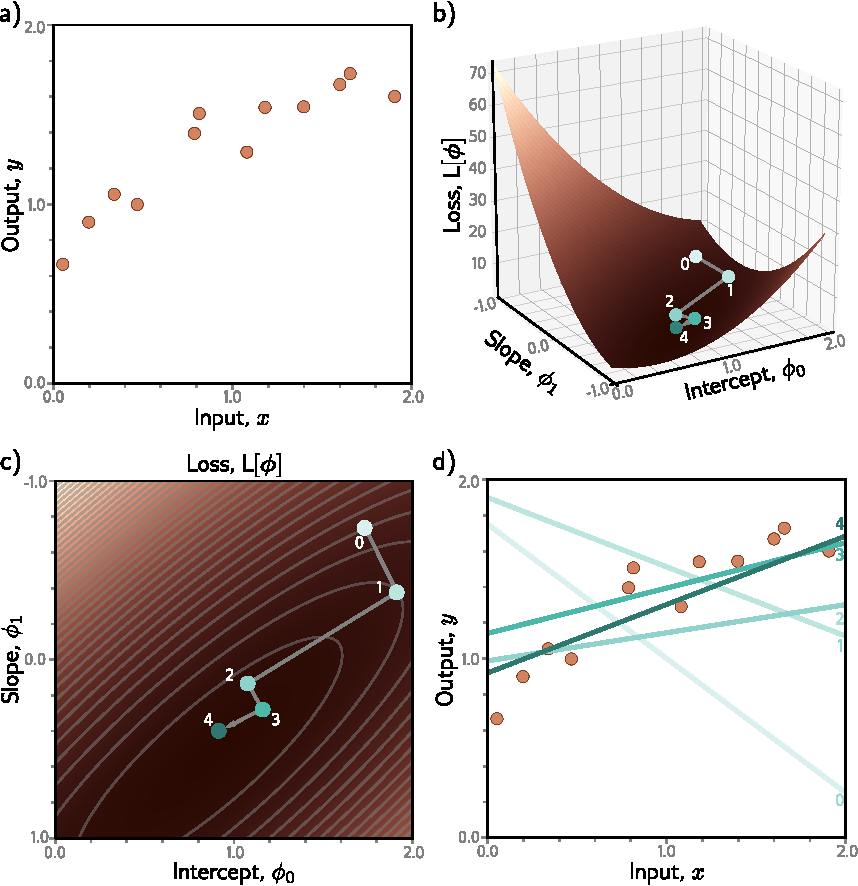
\includegraphics[height=0.665\textheight]{TrainLRMin}
      \end{center}
    \end{column}
    \begin{column}{0.51\textwidth}
      \vspace{0.4em}
      \begin{itemize}\itemsep0.45em
        \item (a) the training set; (b) the loss surface, four
              iterations marked
        \item (c) the same iterations as a heat map
        \item (d) the fitted line at each, lightest first
        \item Least squares for a \alert{linear} model is convex, so
              this cannot fail
      \end{itemize}
      \vspace{0.5em}
      {\scriptsize\color{mcMuted} Prince (2023), Fig.~6.1. His $\phi_0, \phi_1$ are our $w_0, w_1$.}
    \end{column}
  \end{columns}
\end{frame}
\begin{frame}{Two ways to choose the step length}
  \begin{columns}[T, onlytextwidth]
    \begin{column}{0.485\textwidth}
      \textbf{A fixed learning rate}\vspace{0.35em}
      \begin{itemize}\itemsep0.3em
        \item $\eta$ chosen once, before training
        \item One gradient evaluation per step
        \item The only affordable option once $W$ is large
      \end{itemize}
    \end{column}
    \begin{column}{0.485\textwidth}
      \textbf{A line search}\vspace{0.35em}
      \begin{itemize}\itemsep0.3em
        \item Try several $\eta$ and keep the best
        \item Many evaluations per step
        \item Extracts the most progress available along this direction
      \end{itemize}
    \end{column}
  \end{columns}
  \vspace{0.8em}
  \begin{redhighlight}
    A line search is exact and unaffordable; a fixed $\eta$ is crude and
    cheap. Deep learning takes the cheap one and spends the saving on
    many more steps.
  \end{redhighlight}
  \srcline{Prince (2023), \S6.1.}
\end{frame}

\begin{frame}{Choosing the step length by search}
  \begin{center}
    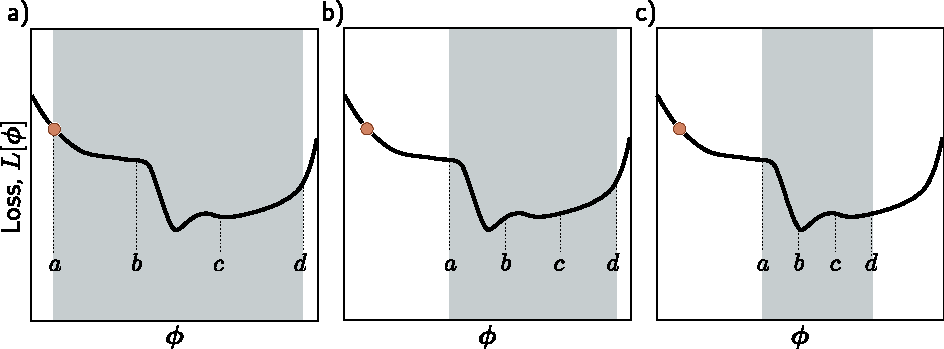
\includegraphics[height=0.55\textheight]{TrainLineSearch}
  \end{center}
  \figcap[0.97]{A line search evaluates several step lengths along the descent direction and keeps the one that lowers the loss most. Prince (2023), \S6.1.}
\end{frame}
\begin{frame}{Four regimes for the step size}
  \vspace{0.3em}
  {\footnotesize
  \renewcommand{\arraystretch}{1.42}
  \begin{tabular}{@{}l@{\hspace{1.8em}}l@{\hspace{1.8em}}l@{}}
    \textbf{Stride} & \textbf{Condition} & \textbf{What happens}\\
    tiny & $\eta \ll 1/L$ & every step helps, but barely: the hiker
      crawls\\
    right & $\eta = 1/L$ & the guaranteed decrease is largest\\
    long & $1/L < \eta < 2/L$ & still downhill, and it starts to
      oscillate\\
    too long & $\eta > 2/L$ & the step overshoots the bend and $E$ can
      \alert{increase}\\
  \end{tabular}}
  \vspace{0.9em}

  \begin{itemize}\itemsep0.35em
    \item Nobody knows $L$ for a deep network, so $\eta$ is tuned by
          experiment
    \item A loss that diverges is the symptom of having crossed $2/L$,
          which is why lowering $\eta$ is the first thing to try
  \end{itemize}
\end{frame}

\begin{frame}{Why gradients are worth their cost}
  \bridge{The surface near a minimum is described by $b$ and $H$, so
  locating it means pinning those down.}
  \vspace{-0.55em}
  \[
    \underbrace{W}_{\text{entries of } b}
    \;+\;
    \underbrace{\tfrac{W(W+1)}{2}}_{\text{independent entries of the symmetric } H}
    \;=\; \frac{W(W+3)}{2} \;=\; O(W^2) \ \text{numbers}
  \]
  \vspace{-0.85em}
  \begin{itemize}\itemsep0.3em
    \item \alert{Function values only}: one number per evaluation, so
          $O(W^2)$ evaluations at $O(W)$ work each
          $\Rightarrow O(W^3)$
    \item \alert{Gradients}: $W$ numbers per evaluation, so $O(W)$
          evaluations, each $O(W)$ by backpropagation
          $\Rightarrow O(W^2)$
  \end{itemize}
  \begin{redhighlight}
    A factor of $W$ --- for a million parameters, a factor of a million.
    \figsource{B\&B (2024), \S7.2.1.}
  \end{redhighlight}
\end{frame}

\begin{frame}{The local quadratic model}
  \bridge{Convexity tells us where we are going. Curvature tells us how
  large a step is safe.}
  \vspace{-0.35em}
  \[
    E(w) \;\simeq\; E(\hat w) + (w - \hat w)^{\mathsf T} b
          + \tfrac12 (w - \hat w)^{\mathsf T} H (w - \hat w),
  \]
  \vspace{-1.0em}
  \[
    b \equiv \nabla E \big|_{w = \hat w},
    \qquad
    H(\hat w) \equiv \nabla\nabla E(w) \big|_{w = \hat w} .
  \]
  \vspace{-0.5em}
  \begin{itemize}\itemsep0.35em
    \item $b$ has length $W$; $H$ is $W \times W$ and symmetric
    \item At a minimum $w^\star$ the linear term vanishes, leaving
          $E(w) = E(w^\star)
           + \tfrac12 (w-w^\star)^{\mathsf T} H (w-w^\star)$
    \item Everything in this section is read off that one expression
  \end{itemize}
  \srcline{Bishop \& Bishop (2024), Eqs.~7.3--7.7.}
\end{frame}

\begin{frame}{Rotating into the eigenvectors of $H$}
  \vspace{0.1em}
  With $H u_i = \lambda_i u_i$ and $u_i^{\mathsf T} u_j = \delta_{ij}$,
  expand the displacement as
  $w - w^\star = \sum_i \alpha_i u_i$. Then
  \vspace{-0.35em}
  \[
    E(w) \;=\; E(w^\star) + \tfrac12 \sum_i \lambda_i \alpha_i^2 .
  \]
  \vspace{-0.6em}
  \begin{itemize}\itemsep0.35em
    \item A change of coordinates: origin at $w^\star$, axes along the
          eigenvectors
    \item Every cross term cancels, by orthonormality
  \end{itemize}
  \begin{redhighlight}
    In these coordinates $E$ is a \emph{sum of independent
    one-dimensional parabolas}, one per eigenvector, the $i$th with
    curvature $\lambda_i$. Nothing couples them.
  \end{redhighlight}
  \srcline{Bishop \& Bishop (2024), Eqs.~7.8--7.11.}
\end{frame}

\begin{frame}{Reading the curvature off the contours}
  \begin{center}
    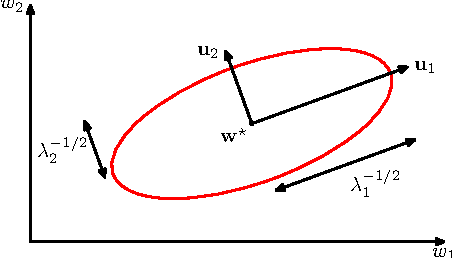
\includegraphics[height=0.56\textheight]{Bishop7_2}
  \end{center}
  \figcap[0.97]{Contours of the quadratic model are ellipses centred on $w^\star$, with axes along the eigenvectors $u_i$ of $H$ and semi-axis lengths proportional to $\lambda_i^{-1/2}$. Bishop \& Bishop (2024), Fig.~7.2.}
\end{frame}
\begin{frame}{Smoothness: one number for the worst curvature}
  \begin{block}{Definition ($L$-smooth)}
    $E$ is \alert{$L$-smooth} if its gradient is Lipschitz,
    \[
      \|\nabla E(u) - \nabla E(v)\| \;\leq\; L \|u - v\|
      \qquad \forall\, u, v .
    \]
  \end{block}
  \vspace{0.3em}
  \begin{itemize}\itemsep0.35em
    \item Equivalently, wherever $E$ is twice differentiable, every
          eigenvalue satisfies $|\lambda_i| \leq L$: it is the
          \alert{sharpest bend anywhere} in the landscape
    \item For a quadratic the curvature is the same everywhere, so
          $L = \lambda_{\max}$ --- the curvature of the sharpest
          cross-section, and the \emph{shortest} axis of the ellipse
    \item $L$ is a property of the \alert{problem}: we do not choose it,
          and in a network we do not know it
  \end{itemize}
\end{frame}

\begin{frame}{How far a single step may go}
  \vspace{-0.25em}
  \begin{lemmax}[One step is guaranteed to go downhill]\label{th:desc}
    \small
    Let $E$ be $L$-smooth and let $w^+ = w - \eta\,\nabla E(w)$. Then
    \[
      E(w^+) \;\leq\; E(w)
        - \eta\Big(1 - \tfrac{L\eta}{2}\Big)\,\|\nabla E(w)\|^2 .
    \]
    In particular $E(w^+) < E(w)$ whenever $0 < \eta < 2/L$ and
    $\nabla E(w) \neq 0$; the bound is tightest at $\eta = 1/L$.
  \end{lemmax}
  {\footnotesize
  \begin{itemize}\itemsep0.26em
    \item \focus{1}{$L$-smoothness gives $E(v) \leq E(w) +
          (v-w)^{\mathsf T}\nabla E(w) + \tfrac{L}{2}\|v-w\|^2$.}
    \item \focus{2}{Put $v = w^+$, so $v - w = -\eta\nabla E(w)$:
          $E(w^+) \leq E(w) - \eta\|\nabla E\|^2
          + \tfrac{L\eta^2}{2}\|\nabla E\|^2$.}
    \item \focus{3}{Collecting the $\|\nabla E\|^2$ terms gives the
          bound; $\eta(1 - L\eta/2) > 0$ on $(0, 2/L)$ and is maximal at
          $\eta = 1/L$. \hfill $\square$}
  \end{itemize}}
  \vspace{-0.35em}
  \srcline{Nesterov (2004), Lemma 1.2.3.}
\end{frame}

\begin{frame}{Removing the assumption}
  \bridge{Everything so far assumed a convex loss. Shallow and deep
  networks are not convex.}
  \vspace{0.5em}
  \begin{itemize}\itemsep0.45em
    \item The steepest-descent lemma survives: it is local, and uses only
          $\nabla E$
    \item The descent lemma survives: it is local, and uses only
          smoothness
    \item What does \alert{not} survive is the link between
          ``stationary'' and ``best''
  \end{itemize}
  \vspace{0.7em}
  \begin{redhighlight}
    Each step is still guaranteed to lower $E$. Nothing guarantees any
    more that the point it converges to is the one we wanted.
  \end{redhighlight}
  \srcline{Prince (2023), \S6.1.2.}
\end{frame}

\begin{frame}{A two-parameter model we can draw}
  \begin{center}
    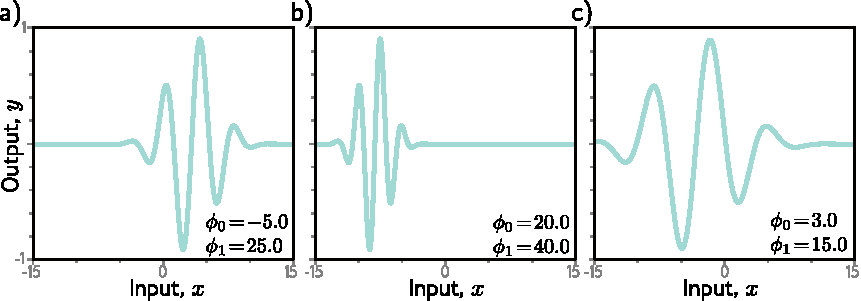
\includegraphics[height=0.52\textheight]{TrainGaborModel}
  \end{center}
  \figcap[0.97]{A model with two parameters: $w_0$ moves it, $w_1$ squeezes it. Prince (2023), Fig.~6.2, where these are $\phi_0$ and $\phi_1$.}
\end{frame}
\begin{frame}{Its training set}
  \begin{center}
    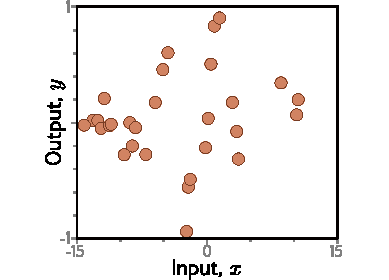
\includegraphics[height=0.50\textheight]{TrainGaborData}
  \end{center}
  \figcap[0.97]{28 points, made by sampling the model at $w = [0.0,\, 16.6]^{\mathsf T}$ and adding Gaussian noise. Prince (2023), Fig.~6.3.}
\end{frame}
\begin{frame}{A loss that is not convex}
  \vspace{0.2em}
  \begin{columns}[T, onlytextwidth]
    \begin{column}{0.46\textwidth}
      \begin{center}
        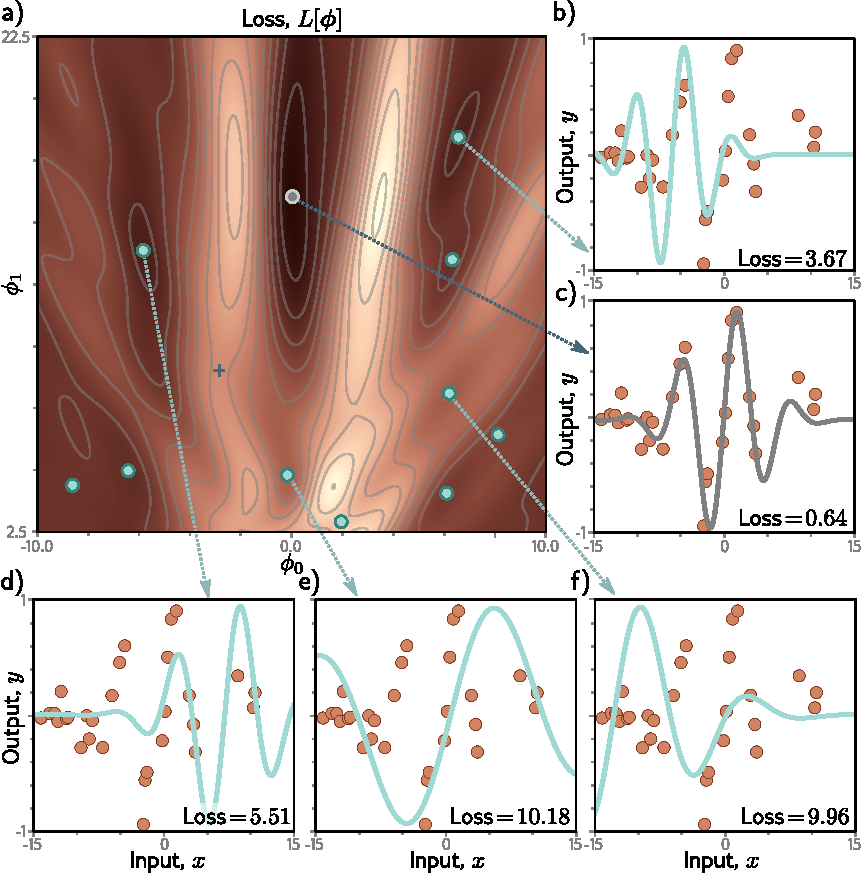
\includegraphics[height=0.665\textheight]{TrainGaborMin}
      \end{center}
    \end{column}
    \begin{column}{0.51\textwidth}
      \vspace{0.4em}
      \begin{itemize}\itemsep0.45em
        \item (a) \alert{many local minima} (cyan), one global
              minimum (grey)
        \item The blue cross is a \alert{saddle point}: $\nabla E = 0$,
              but the surface falls away in one direction
        \item (b)--(f) are the models at each minimum; none improves
              under a small change
      \end{itemize}
      \vspace{0.5em}
      {\scriptsize\color{mcMuted} Prince (2023), Fig.~6.4.}
    \end{column}
  \end{columns}
\end{frame}
\begin{frame}{Stationary points}
  \vspace{-0.2em}
  \begin{propx}[Classification of stationary points]\label{th:sig}
    \small
    Let $\nabla E(w^\star) = 0$ and let $H$ be the Hessian at $w^\star$,
    with eigenvalues $\{\lambda_i\}$. Then $w^\star$ is a local minimum
    if and only if $\lambda_i > 0$ for all $i$; a local maximum if and
    only if $\lambda_i < 0$ for all $i$; and a saddle point if the signs
    are mixed.
  \end{propx}
  \vspace{0.1em}
  {\footnotesize
  \begin{itemize}\itemsep0.28em
    \item \focus{1}{Fix $j$, set $\alpha_i = 0$ for $i \neq j$ and vary
          $\alpha_j$: then $E - E(w^\star) =
          \tfrac12 \lambda_j \alpha_j^2$.}
    \item \focus{2}{So each eigen-direction votes independently: $E$
          rises along $u_j$ if $\lambda_j > 0$ and falls if
          $\lambda_j < 0$.}
    \item \focus{3}{Writing $v = \sum_i c_i u_i$ gives
          $v^{\mathsf T} H v = \sum_i c_i^2 \lambda_i$, so $H$ is
          positive definite exactly when every $\lambda_i > 0$.}
    \item \focus{4}{That is the condition for a minimum.
          \hfill $\square$}
  \end{itemize}}
  \vspace{-0.3em}
  \srcline{Bishop \& Bishop (2024), \S7.1.1.}
\end{frame}

\begin{frame}{Saddle points are the practical problem}
  \vspace{0.3em}
  \begin{itemize}\itemsep0.45em
    \item At a saddle the gradient vanishes, but the surface falls away
          in at least one direction
    \item Gradient descent can leave a saddle --- provided it is not
          sitting exactly on it
    \item But the surface nearby is \alert{flat}, so
          $\|\nabla E\|$ is small over a large region
    \item Stopping when $\|\nabla E\|$ is small therefore risks stopping
          at a saddle and calling it convergence
    \item In high dimension saddles vastly outnumber local minima: a
          random sign pattern is far more likely to be mixed than all
          positive
  \end{itemize}
  \srcline{Prince (2023), \S6.1.3.}
\end{frame}

\begin{frame}{How many minima are there?}
  \vspace{0.3em}
  \begin{itemize}\itemsep0.45em
    \item A two-layer network with $M$ hidden units has $M!\,2^M$
          parameter vectors computing the \alert{same} function
    \item So every minimum arrives with a combinatorial family of copies
          --- for $M = 100$, more than $10^{187}$ of them
    \item Beyond those there are \alert{non-equivalent} minima: one
          global, many local. It was long feared these would trap
          gradient methods; in practice large networks reach comparable
          solutions from many different starts
  \end{itemize}
  \begin{redhighlight}
    Counting minima is the wrong worry. Their \emph{quality} is the right
    one.
  \end{redhighlight}
  \srcline{Bishop \& Bishop (2024), \S6.2.4, \S7.1.}
\end{frame}

\begin{frame}{The bill for losing convexity}
  \vspace{0.3em}
  {\footnotesize
  \renewcommand{\arraystretch}{1.42}
  \begin{tabular}{@{}l@{\hspace{1.6em}}l@{}}
    \textbf{On a convex loss} & \textbf{On a network's loss}\\
    every stationary point is global & stationary says nothing about
      quality\\
    the destination is the best solution & the destination is decided by
      the start\\
    small $\|\nabla E\|$ means nearly done & it may mean a saddle\\
    one run suffices & several runs, compared on held-out data\\
  \end{tabular}}
  \vspace{0.9em}

  \begin{redhighlight}
    Deterministic descent inherits every flaw of the point it was
    dropped at. The remedy in the next section is not a better direction
    --- it is a \emph{noisier} one.
  \end{redhighlight}
\end{frame}

% =====================================================================
\section{Stochastic and Mini-batch Gradient Descent}
% =====================================================================

\begin{frame}{The cost of a batch step}
  \vspace{0.3em}
  \begin{itemize}\itemsep0.45em
    \item $E(w) = \sum_{n=1}^{N} E_n(w)$, so one gradient costs $N$
          backward passes
    \item With $N$ in the millions, a single parameter update becomes a
          major computation
    \item It is also \alert{wasteful under redundancy}: duplicate every
          data point and the cost doubles while the direction is
          unchanged, up to a rescaling of $\eta$
  \end{itemize}
  \begin{redhighlight}
    We do not need the exact gradient. We need a cheap direction that is
    right \emph{on average}.
  \end{redhighlight}
  \srcline{Bishop \& Bishop (2024), \S7.2.3.}
\end{frame}

\begin{frame}{Stochastic gradient descent}
  \vspace{-0.3em}
  \[
    w^{(\tau)} \;=\; w^{(\tau-1)}
      - \eta\, \nabla E_n\!\left(w^{(\tau-1)}\right)
  \]
  \vspace{-0.85em}
  \begin{itemize}\itemsep0.3em
    \item One data point per update; a full pass over the data is an
          \alert{epoch}
    \item Also called \emph{online} gradient descent when the data
          arrives as a stream
  \end{itemize}
  \vspace{0.35em}
  \begin{algox}[Stochastic gradient descent]\label{th:sgd}
    \small
    \textbf{Input:} data indexed by $n \in \{1,\dots,N\}$; per-point
    error $E_n(w)$; learning rate $\eta$; initial $w$\\[0.25em]
    $n \leftarrow 1$;\quad
    \textbf{repeat}\quad
      $w \leftarrow w - \eta \nabla E_n(w)$;\quad
      $n \leftarrow n + 1 \pmod N$\\
    \textbf{until} convergence;\quad \textbf{return} $w$
  \end{algox}
  \srcline{Bishop \& Bishop (2024), Eq.~7.18, Alg.~7.1; Bottou (2010).}
\end{frame}

\begin{frame}{The estimate is unbiased}
  \vspace{-0.2em}
  \begin{propx}[Mean and variance of the mini-batch gradient]\label{th:mb}
    \small
    Let $\mathcal{B}$ be $B$ indices drawn uniformly at random and let
    $\hat g = \tfrac{N}{B} \sum_{n \in \mathcal{B}} \nabla E_n(w)$. Then
    $\mathbb{E}[\hat g] = \nabla E(w)$, and each component of $\hat g$
    has standard deviation $N\sigma/\sqrt{B}$, where $\sigma$ is the
    standard deviation of that component across the data.
  \end{propx}
  \vspace{0.1em}
  {\footnotesize
  \begin{itemize}\itemsep0.28em
    \item \focus{1}{Each index is uniform on $\{1,\dots,N\}$, so
          $\mathbb{E}[\nabla E_n] = \tfrac1N \nabla E$.}
    \item \focus{2}{Linearity over the $B$ draws gives
          $\mathbb{E}[\hat g] = \tfrac{N}{B}\, B\, \tfrac1N \nabla E
          = \nabla E$: \alert{unbiased, for every $B$}.}
    \item \focus{3}{$\hat g$ is $N$ times a sample mean of $B$ draws, so
          its variance is $N^2\sigma^2/B$.}
    \item \focus{4}{The $\sqrt{B}$ in the denominator is the whole
          argument for mini-batches. \hfill $\square$}
  \end{itemize}}
  \vspace{-0.3em}
  \srcline{Bishop \& Bishop (2024), \S7.2.4; Prince (2023), \S6.2.1.}
\end{frame}

\begin{frame}{Each batch is its own surface}
  \vspace{0.2em}
  \begin{columns}[T, onlytextwidth]
    \begin{column}{0.46\textwidth}
      \begin{center}
        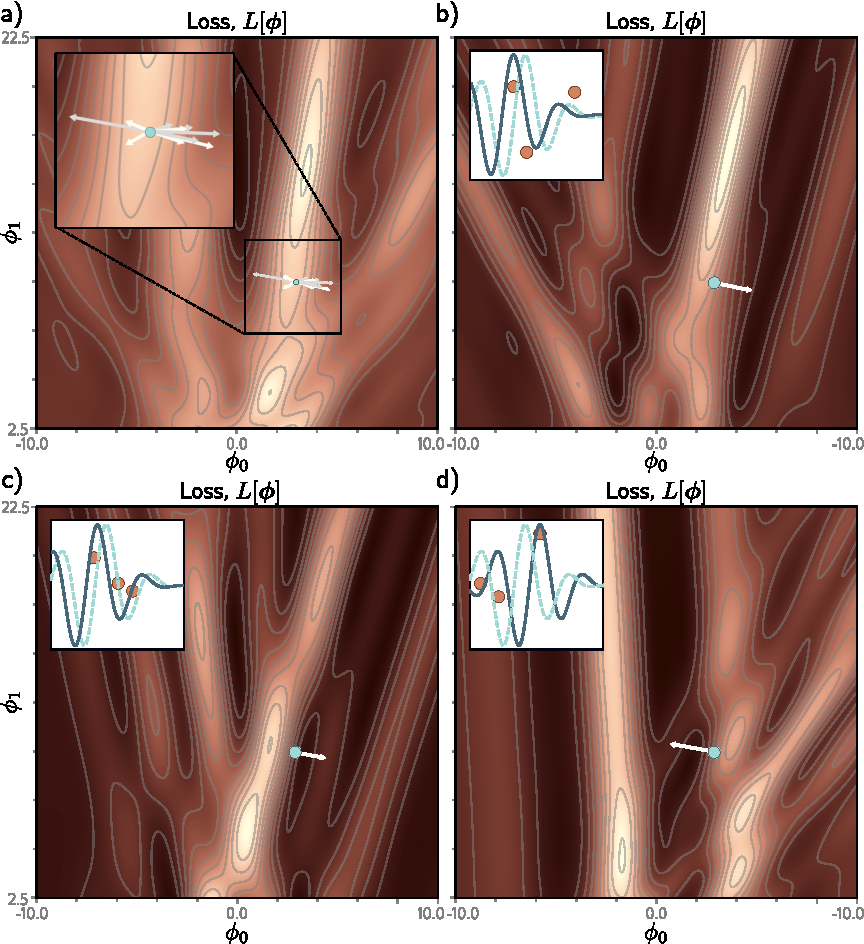
\includegraphics[height=0.665\textheight]{TrainGaborSGDIter}
      \end{center}
    \end{column}
    \begin{column}{0.51\textwidth}
      \vspace{0.4em}
      \begin{itemize}\itemsep0.45em
        \item (a) the full loss, with the distribution of possible
              updates inset
        \item (b), (c) two batches, each with its own surface and its
              own downhill direction
        \item (d) a step that goes \alert{downhill on the batch but
              uphill on the full loss}
      \end{itemize}
      \vspace{0.5em}
      {\scriptsize\color{mcMuted} Prince (2023), Fig.~6.6.}
    \end{column}
  \end{columns}
\end{frame}
\begin{frame}{Mini-batches}
  \vspace{-0.35em}
  \[
    w^{(\tau)} \;=\; w^{(\tau-1)}
      - \eta \sum_{n \in \mathcal{B}_\tau}
        \nabla E_n\!\left(w^{(\tau-1)}\right)
  \]
  \vspace{-0.7em}
  \begin{itemize}\itemsep0.35em
    \item $B = 1$ is stochastic gradient descent, $B = N$ is batch
          descent, and everything useful lies in between
    \item Raising $B$ a hundredfold improves the estimate tenfold and
          costs a hundredfold --- \alert{diminishing returns}
    \item Powers of two are common because they suit the hardware
  \end{itemize}
  \begin{redhighlight}
    The name does not change: it is still called ``stochastic gradient
    descent'' when $B > 1$.
    \figsource{Prince (2023), Eq.~6.10; B\&B (2024), \S7.2.4.}
  \end{redhighlight}
\end{frame}

\begin{frame}{Mini-batch stochastic gradient descent}
  \vspace{0.2em}
  \begin{algox}[Mini-batch stochastic gradient descent]\label{th:msgd}
    \small
    \textbf{Input:} data indexed by $n \in \{1,\dots,N\}$; batch size
    $B$; per-batch error $E_{n:n+B-1}(w)$; learning rate $\eta$;
    initial $w$\\[0.35em]
    $n \leftarrow 1$\\
    \textbf{repeat}\\
    \hspace{1.4em} $w \leftarrow w - \eta \nabla E_{n:n+B-1}(w)$
      \hfill \textcolor{mcMuted}{// weight vector update}\\
    \hspace{1.4em} $n \leftarrow n + B$\\
    \hspace{1.4em} \textbf{if} $n > N$ \textbf{then}
      \; shuffle data; \; $n \leftarrow 1$ \; \textbf{end if}\\
    \textbf{until} convergence\\
    \textbf{return} $w$
  \end{algox}
  \srcline{Bishop \& Bishop (2024), Algorithm 7.2.}
\end{frame}

\begin{frame}{What the batch size buys}
  \vspace{0.3em}
  \begin{itemize}\itemsep0.45em
    \item A small batch does not converge to a point; it settles into a
          \alert{noise ball} whose radius grows as $B$ shrinks
    \item Per \emph{iteration} the full batch wins --- it has the exact
          direction
    \item Per \emph{gradient evaluation}, which is what costs money, a
          small batch is far ahead early
    \item The crossover is why practice uses a mini-batch, then raises
          $B$ or lowers $\eta$ late in training
  \end{itemize}
  \begin{redhighlight}
    Choosing $B$ is choosing where on this trade-off to sit, which is
    exactly why $B$ is a hyperparameter and not a derived quantity.
  \end{redhighlight}
\end{frame}

\begin{frame}{Shuffling}
  \vspace{0.3em}
  \begin{itemize}\itemsep0.45em
    \item Raw data sets carry an order: collected by date, sorted
          alphabetically, grouped by class
    \item Consecutive blocks then make every batch unrepresentative, and
          Proposition~\ref{th:mb} no longer applies --- the draw is not
          uniform
    \item Shuffle the whole set, then take batches as successive blocks
    \item Reshuffling between epochs means a batch is unlikely to repeat,
          which also helps leave a poor valley
  \end{itemize}
  \begin{redhighlight}
    Unbiasedness was assumed, not granted. Shuffling is what makes the
    assumption true.
  \end{redhighlight}
\end{frame}

\begin{frame}{Noise is the feature}
  \begin{center}
    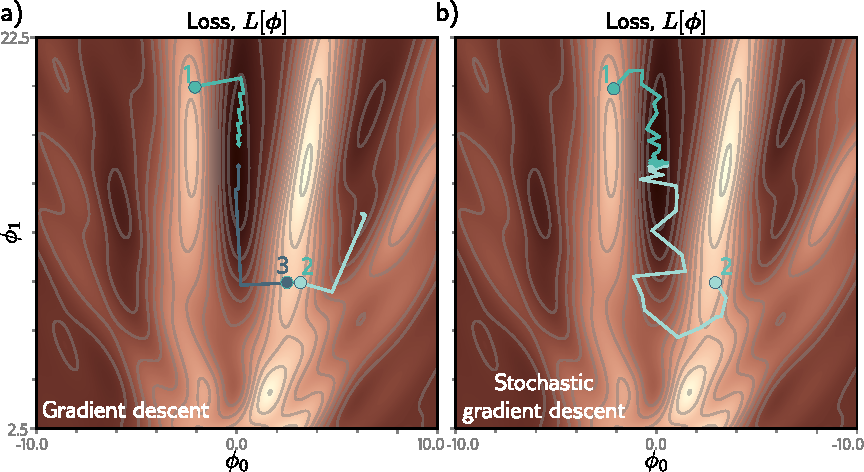
\includegraphics[height=0.56\textheight]{TrainGaborGDSGD}
  \end{center}
  \figcap[0.97]{(a) gradient descent, whose destination is fixed by the start; (b) stochastic gradient descent, which can leave the wrong valley. Prince (2023), Fig.~6.5.}
\end{frame}
\begin{frame}{Six properties of stochastic gradient descent}
  \vspace{0.1em}
  {\footnotesize
  \begin{enumerate}\itemsep0.36em
    \item It still improves the fit \alert{to some subset} at every step,
          so the updates are sensible even when they are not optimal
    \item Drawing without replacement means every example contributes
          equally over an epoch
    \item It is cheaper per step by a factor of $N/B$
    \item It can \alert{escape local minima}: a stationary point of $E$
          is generally not a stationary point of any $E_n$
    \item It is less likely to stall near a saddle --- some batch will
          have a real gradient there
    \item There is evidence that the solutions it finds
          \alert{generalize} better, which we return to in Class 18
  \end{enumerate}}
  \srcline{Prince (2023), \S6.2.2; Bishop \& Bishop (2024), \S7.2.3.}
\end{frame}

\begin{frame}{One honest caveat}
  \vspace{0.2em}
  \begin{itemize}\itemsep0.45em
    \item SGD does not converge in the classical sense: with a fixed
          $\eta$ the iterate never stops moving
    \item The hope is that near a good solution every batch is well
          fitted, so every batch gradient is small
    \item In the next class we ask when that hope is justified, and add
          memory of past steps and a schedule for $\eta$
  \end{itemize}
  \vspace{0.35em}
  \bspar{exact direction, expensive, destination fixed by the start}
        {noisy direction, cheap, can change valley}
  \begin{redhighlight}
    This section rests on one substitution: replace $\nabla E$ by
    something with the \emph{same mean} and a manageable variance.
  \end{redhighlight}
\end{frame}

% =====================================================================
\section{Putting It Together}
% =====================================================================

\begin{frame}{One training run, end to end}
  \vspace{0.5em}
  \begin{center}
  \begin{tikzpicture}[>=Stealth, line width=0.9pt, font=\small,
      scale=0.88, transform shape,
      b/.style={rounded corners=3pt, draw=shc, fill=shc!7,
                align=center, minimum height=0.95cm,
                inner xsep=4pt, font=\footnotesize},
      d/.style={rounded corners=3pt, draw=dpc, fill=dpc!7,
                align=center, minimum height=0.95cm,
                inner xsep=4pt, font=\footnotesize},
      g/.style={rounded corners=3pt, draw=accc, fill=accc!10,
                align=center, minimum height=0.95cm,
                inner xsep=4pt, font=\footnotesize}]
    \node[g] (init) {initialize $w$};
    \node[b, right=5mm of init] (sh)  {shuffle\\ the data};
    \node[b, right=5mm of sh]   (bat) {take a batch\\ of size $B$};
    \node[b, right=5mm of bat]  (fwd) {forward pass\\ $\to E_{\mathcal{B}}$};
    \node[d, right=5mm of fwd]  (bwd) {backward pass\\ $\to \nabla E_{\mathcal{B}}$};
    \node[d, right=5mm of bwd]  (upd) {$w \leftarrow w - \eta \nabla E_{\mathcal{B}}$};
    \foreach \a/\b in {init/sh, sh/bat, bat/fwd, fwd/bwd, bwd/upd}
      \draw[->] (\a) -- (\b);
    \draw[->, dpc] (upd.south) -- ++(0,-0.72)
      -| node[pos=0.25, below, font=\scriptsize, mcMuted]
      {next batch, and reshuffle at the end of each epoch} (bat.south);
  \end{tikzpicture}
  \end{center}
  \vspace{0.4em}
  \begin{itemize}\itemsep0.3em
    \item Only the maroon boxes are new today, and only the last one is
          a choice
  \end{itemize}
\end{frame}

\begin{frame}{What we choose, and what chooses itself}
  \vspace{0.35em}
  {\footnotesize
  \renewcommand{\arraystretch}{1.40}
  \begin{tabular}{@{}l@{\hspace{1.6em}}l@{\hspace{1.6em}}l@{}}
    \textbf{Quantity} & \textbf{Set by} & \textbf{Governed by}\\
    $\nabla E$ & the model and the data & backpropagation\\
    $L$ & the problem & nothing we control\\
    $\eta$ & \alert{us} & must satisfy $\eta < 2/L$
      (Lemma~\ref{th:desc})\\
    $B$ & \alert{us} & noise $\propto 1/\sqrt{B}$, cost $\propto B$
      (Prop.~\ref{th:mb})\\
    shuffling & \alert{us} & required for Proposition~\ref{th:mb}\\
    $w^{(0)}$ & \alert{us} & taken up in Class 15\\
  \end{tabular}}
  \vspace{0.9em}

  \begin{redhighlight}
    Four of the six rows are ours to choose, and today gives a principled
    reason for three of them.
  \end{redhighlight}
\end{frame}

\begin{frame}{Takeaways}
  \vspace{0.15em}
  {\footnotesize
  \begin{enumerate}\itemsep0.38em
    \item On a convex loss descent cannot fail: every stationary point
          is global, wherever we start
    \item $-\nabla E$ is the steepest descent direction, and uniquely so
          (Lemma~\ref{th:steep})
    \item The eigenvalues of $H$ are curvatures; $\lambda_{\max}$ is the
          sharpest one, and it sets $L$
    \item A step with $\eta < 2/L$ is guaranteed to lower $E$; a larger
          one can raise it (Lemma~\ref{th:desc})
    \item Gradients are worth their cost by a factor of $W$
    \item Losing convexity costs the link between ``stationary'' and
          ``best''; saddles, not local minima, are the practical
          difficulty
    \item The mini-batch gradient is unbiased with standard error
          $\propto 1/\sqrt{B}$ (Prop.~\ref{th:mb}), and its noise is what
          stops the starting point being destiny
  \end{enumerate}}
  \bridge{Next class: the step is safe, but how fast does it arrive?}
\end{frame}

\begin{frame}{References}
  \vspace{0.25em}
  {\scriptsize
  \begin{itemize}\itemsep0.30em
    \item C.~M. Bishop \& H. Bishop, \emph{Deep Learning: Foundations
          and Concepts}, Springer, 2024. Chapter 7, \S7.1--7.2
          (Eqs.~7.1--7.18, Algorithms 7.1--7.2, Figs.~7.1--7.2).
    \item S.~J.~D. Prince, \emph{Understanding Deep Learning}, MIT
          Press, 2023. Chapter 6, \S6.1--6.2 (Eqs.~6.1--6.10,
          Figs.~6.1--6.6); \S7.1.
    \item L. Bottou, ``Large-scale machine learning with stochastic
          gradient descent'', \emph{COMPSTAT}, 2010.
    \item Y. Nesterov, \emph{Introductory Lectures on Convex
          Optimization}, Kluwer, 2004.
    \item H. Robbins \& S. Monro, ``A stochastic approximation method'',
          \emph{Annals of Mathematical Statistics}, 1951.
  \end{itemize}}
\end{frame}

\begin{frame}[standout]
  Questions?
\end{frame}

\end{document}
